At the component level, the scheduling semantics often can be directly modelled in the AADL AGREE annex. This requires introducing two boolean variables dispatch and complete, augumenting the orignal contracts with dispatch or complete, and adding additional guarantees to enforce the output freeze rule. We often omit the assumptions to enforce the input freeze rule, as they are trivially satisfied by the output freeze rule.
Figure \ref{wpmAGREE} shows an example taken from an AADL model developed in the CASE project. The first two guarantees are added. And the orignal contracts (the assumption and the third guarantee) are augumented. 
It could be complicated to direct model contracts that dependend on past history. We rely on our Lustre backend model to handle the general case.

\begin{figure}[ht!]
\centering
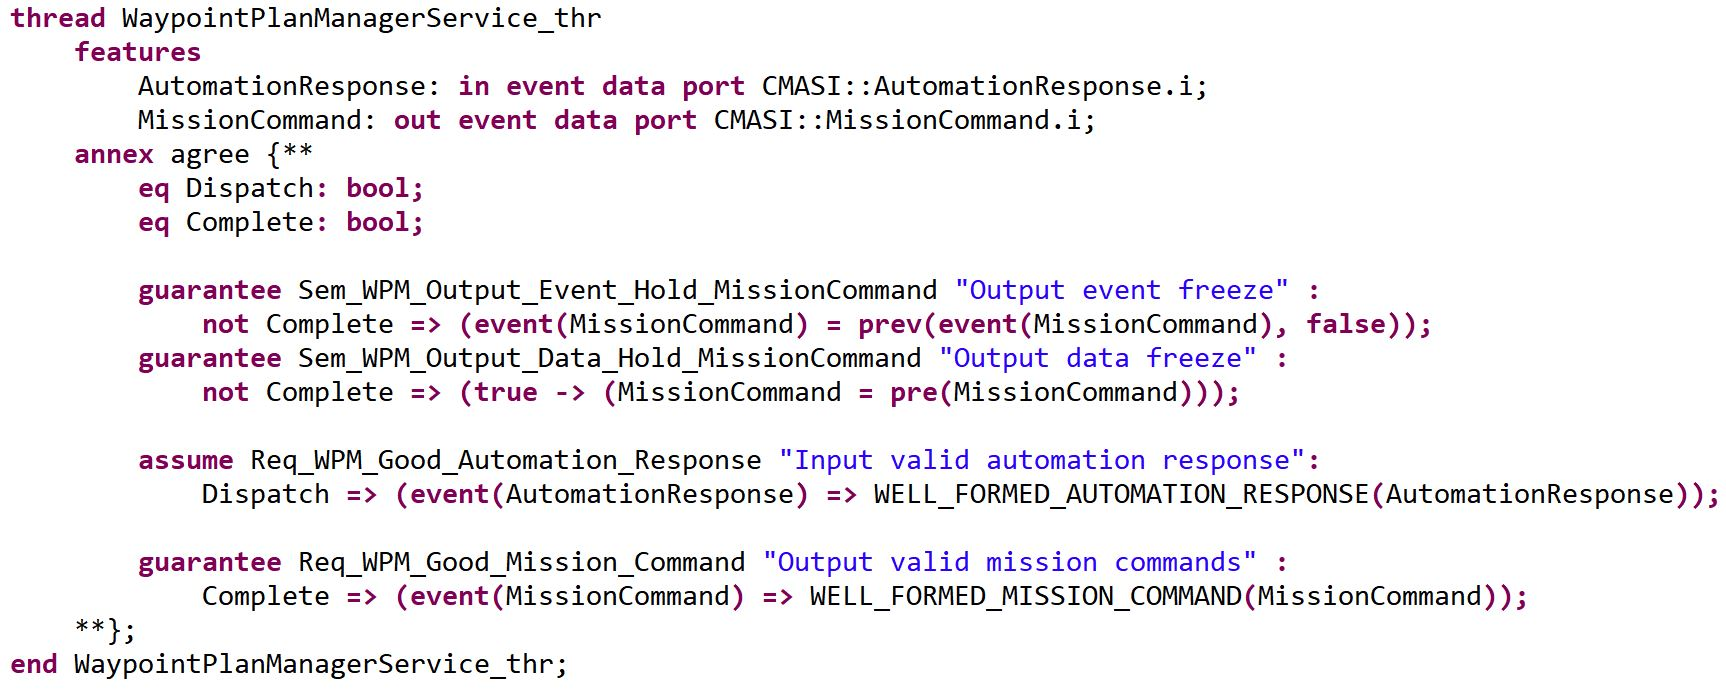
\includegraphics[width=130mm]{wpmAGREE3.jpg}
\caption{Direct Modelling Scheduling Semantics in AGREE\label{wpmAGREE}}
\end{figure}

At the system-level, we use a circular counter to model a cyclic schedule in AGREE. 
The counter updates at every instant. Once it reaches the limit, it resets to 1 in the next instant.
We set the limit to the period of the schedule. 
%The counter is a direct encoding of schedule $\phi$ defined previously.
Then based on the current count, a corresponding scheduling event is raised.
Figure \ref{schedule} shows an AGREE model of the schedule $(ABACD)$.

\begin{figure}[ht!]
\centering
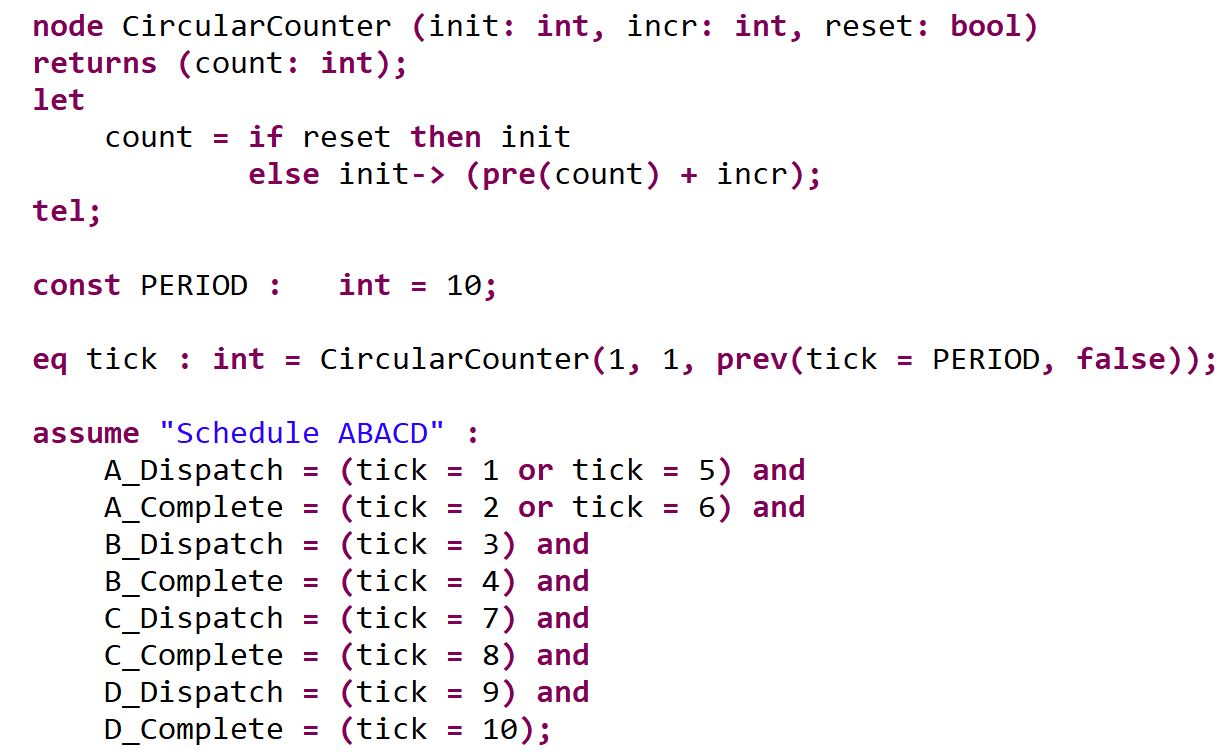
\includegraphics[width=100mm]{schedule.jpg}
\caption{A Model of Schedule in AGREE\label{schedule}}
\end{figure}

%An AGREE model of the schedule $(ABACD)^*$ used in the example is shown in code~\ref{schedule_model}

%\begin{lstlisting}[language=c,frame=single,caption=An AGREE model of a schedule,label=schedule_model]
%node CircularCounter (init: int, incr: int, reset: bool)	
%returns (count: int);
%let
%	count = if reset then init
%		else init-> (pre(count) + incr);
%tel;
%				
%eq tick : int = CircularCounter(1,1,prev(tick=10,false));
%
%assume "Schedule ABACD" :
%	A_dispatch = (tick = 1 or tick = 5) and
%	A_complete = (tick = 2 or tick = 6) and					
%	B_dispatch = (tick = 3) and	
%	B_complete = (tick = 4) and
%	C_dispatch = (tick = 7) and
%	C_complete = (tick = 8) and	
%	D_dispatch = (tick = 9) and
%	D_complete = (tick = 10);			
%\end{lstlisting}	

